\documentclass{prova}

\usepackage{amssymb}
\usepackage{tasks}
\usepackage[inline]{enumitem}

\renewcommand{\sin}{\mbox{sen}}
\newcommand{\ra}{\rightarrow}
\newcommand{\lra}{\leftrightarrow}
\newcommand{\Ra}{\Rightarrow}
\newcommand{\LRa}{\Leftrightarrow}
\renewcommand{\lnot}{\sim}
\newcommand{\larg}{\vdash}

\professor{Prof. Adriano Barbosa}
\disciplina{\'Algebra Elementar}
\avaliacao{PS}
\curso{Matem\'atica}
\data{07/12/2018}

\begin{document}
	\cabecalho{5}  % o numero 5 indica a qnt de quadros na tabela de nota

	\textbf{Todas as respostas devem ser justificadas.}

    \vspace{0.5cm}
    \textbf{Avalia\c{c}\~ao P1:}
	\begin{questionario}
        \q{Dadas as proposi\c{c}\~oes $p:$ Jo\~ao \'e feliz, $q:$ Maria \'e alta. Escreva
        usando a linguagem corrente as proposi\c{c}\~oes abaixo:}
            \begin{questionario}
                \qq{$\lnot p$}
                \qq{$p \land q$}
                \qq{$p \lor q$}
                \qq{$(\lnot p)\ra q$}
            \end{questionario}
        \q{Determine se a equival\^encia $\lnot (p\land q) \LRa\ \lnot p\ \lor
        \lnot q$ \'e v\'alida.}
        \q{Escreva a forma contr\'aria, a contrapositiva e a rec\'{\i}proca da
        proposi\c{c}\~ao $P:$ Se eu n\~ao for ao parque, ent\~ao irei circo.}
        \q{Determine o conjunto verdade das senten\c{c}as abertas:}
            \begin{questionario}
                \qq{$x\in\mathbb{N}$ tal que $2x^2-x=0$}
                \qq{$x\in\mathbb{Z}$ tal que $2x^2-x=0$}
                \qq{$x\in\mathbb{Q}$ tal que $2x^2-x=0$}
                \qq{$x\in\mathbb{R}$ tal que $2x^2-x=0$}
            \end{questionario}
        \q{Mostre que se $mn$ \'e um inteiro \'{\i}mpar, ent\~ao $m$ e $n$ s\~ao ambos
        inteiros \'{\i}mpares.}
	\end{questionario}

    \vspace{0.5cm}
    \textbf{Avalia\c{c}\~ao P2:}
    \begin{questionario}
        \q{Dados $A=\{1,2\}$ e $B=\{1,2,3\}$. Determine se as afirma\c{c}\~oes abaixo s\~ao
        verdadeiras ou falsas:}
            \begin{tasks}[style=enumerate,
            counter-format={(tsk[a])},label-offset={0.25cm}](4)
                \task $1\in A$
                \task $\{1\}\in A$
                \task $\{1\}\subset A$
                \task $\varnothing \in A$
                \task $A\subset B$
                \task $A\in B$
                \task $\varnothing\in\{\varnothing, A\}$
                \task $\varnothing\subset\{\varnothing, A\}$
                \task $\{\varnothing\}\in\{\varnothing, A\}$
                \task $\{\varnothing\}\subset\{\varnothing, A\}$
            \end{tasks}
        \q{Mostre que $(A\cap B)^C = A^C \cup B^C$, quaisquer que sejam os
        conjuntos $A$ e $B$.}
        \q{Use o princ\'{\i}pio de indu\c{c}\~ao para mostrar que}
            \[2^1 + 2^2 + 2^3 + \cdots + 2^n = 2^{n+1}-2, \forall\ n\in\mathbb{N}.\]
        \q{Determine no diagrama de Venn cada um dos conjuntos abaixo:}

            \begin{enumerate*}
                \qq{$A-(B\cap C)$}
                \hspace{1.8cm}
                \hspace{1.8cm}
                \qq{$(A-B)\cup(A-C)$}
            \end{enumerate*}
            \begin{figure}[h]
                \centering
                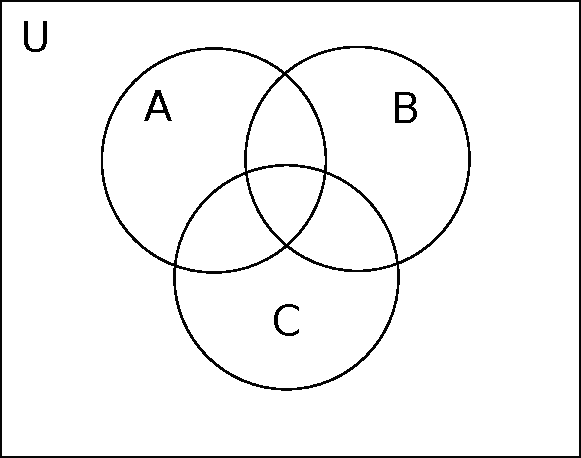
\includegraphics[width=0.4\textwidth]{q4.pdf}
                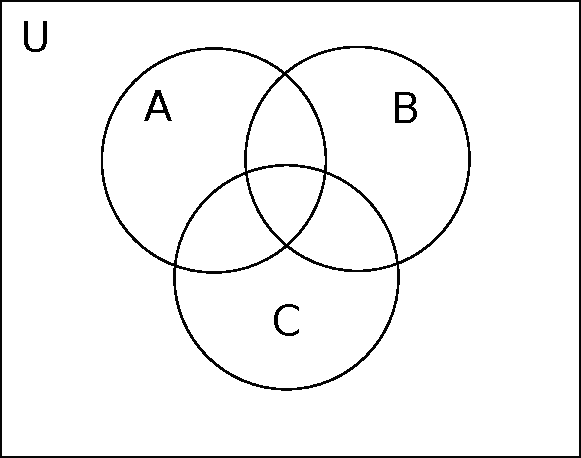
\includegraphics[width=0.4\textwidth]{q4.pdf}
            \end{figure}
        \q{Dados os conjuntos $A=\{-1,0,1\}$ e $B=\{-i,i\}$, determine os elementos de:}
            \begin{questionario}
                \qq{$A \times B$}
                \qq{$B \times A$}
                \qq{$R=\{(x,y)\in A \times A\ |\ x^2+y^2=1\}$}
            \end{questionario}
    \end{questionario}
\end{document}
